\subsection{Model Accuracy Evaluation}\label{sec:model_accuracy_evaluation}

In this section, we present how we used nuggets to identify sources of errors in gem5's models.
Identifying sources of errors in the simulation model is key to establishing baseline performance for evaluating architectural ideas.

Microbenchmarks are a common tool for fine-tuning architectural simulators.
To build a useful model of the Ampere Altra processor, we developed a collection of models including CPU, cache, and memory models using publicly available information on the hardware~\cite{ampere-altra}.
We used a set of microbenchmarks and fine-tuned the configuration of the models to lower the error in simulated cycles~\cite{vertical-microbench}.
While we were able to reduce cycle count error to below 5\% for many of the microbenchmarks, the models struggled to accurately simulate real applications such as NAS Parallel Benchmarks---with errors exceeding 600\%~\cite{npb}.

Using microbenchmarks has two main limitations.
(1) In many cases the compiler optimizations can remove essential parts of the code, resulting in false positives.
% Disabling the compiler optimization is not feasible since it causes other performance regressions such as register pressure.
(2) Even when preserved after compiler optimizations, these microbenchmarks often exercise a narrow slice of the design space, missing the complex interactions between microarchitectural components present in real programs.

While it is possible to develop more sophisticated microbenchmarks, this approach is labor-intensive and does not scale well as architectures develop.
Nuggets are an organic alternative to microbenchmarks;
they capture the diverse instruction mix and control flow found in the real workloads and they are small enough to provide a focused window for manual inspection by the users.

% In the following we describe how we used nuggets from the NAS Parallel benchmarks to identify a source of discrepancy in our models of Ampere Altra processor.

\begin{figure}[!t]
  \centering
  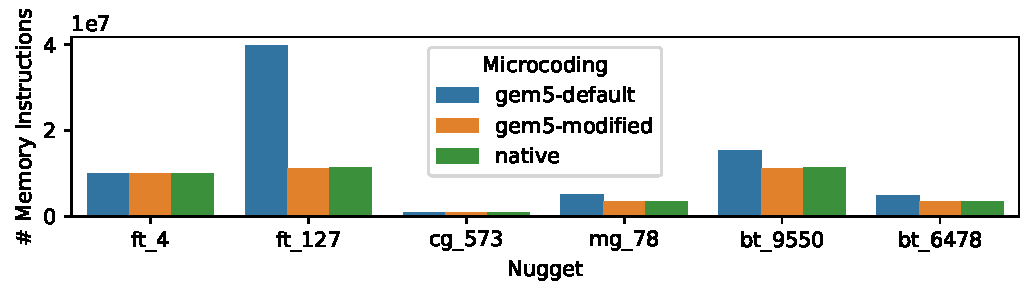
\includegraphics[width=\linewidth]{images/microcode_comp.pdf}
  \caption{Comparison of the number of memory instructions for two different microcodings in gem5 vs.\ real hardware.}
  \label{fig:microcode_comp}
\end{figure}

To improve our model's accuracy, we collected hardware performance counters for 234 nuggets and compared the hardware counters to gem5 statistics for each nugget to identify the nuggets with the largest error.
We found that the data cache statistics explained most of the runtime error and for more than 97\% of the nuggets, the error in the number of accesses to the data cache could be explained by differences in the number of memory instructions.
We isolated the problem by inspecting execution traces from a small set of the nuggets. %---4 randomly selected nuggets and the nuggets with the largest and smallest error in number of memory instructions.
We observed that the nugget with the largest error was dominated by Arm's paired memory instructions (e.g., ldp, stp), while fewer were present in samples with small error.
% However, our microbenchmarks did not exercise these instructions.

Figure~\ref{fig:microcode_comp} shows a comparison of the number of memory instructions in our selected nuggets for three different microcodings.
The orange bars show the number of memory instructions with the default microcoding of gem5;
the blue bars show the number of memory instructions if the paired memory instructions were microcoded as one microop;
while the green bars show the number of memory instructions measured on native hardware.
The blue bars closely track the green bars, suggesting that the microcoding of paired memory instructions in gem5 is different from the native hardware.

% Overall, using microbenchmarks help identify specification errors in simulations models---e.g. when the width of the fetch stage is incorrectly set.
% However, tests using microbenchmarks do not provide enough coverage to identify modeling errors---i.e. errors originating from how models are designed and implemented.
% Nuggets provide an automatic approach to extract rich architectural measurements helping pinpoint modeling errors.
% Modeling errors should be fixed before adjusting for specification errors can help improve the accuracy of the models.

